\section{Desarrollo}

En esta sección vamos a ver en detalle un análisis del desarrollo del proyecto, desde un punto de vista técnico.

\subsection{Prácticas de desarrollo}

Como bien fue mencionado anteriormente, debido a la homogeneidad de los individuos involucrados en este desarrollo, las practicas para poder asegurar la robustez del software fueron abordadas desde el punto de vista de la planificación del proyecto. De esta manera, todas las tareas que involucran pasos críticos de comunicacion son desarrolladas principalmente por el techlead o bien por equipos de desarrollo bajo supervisión directa de este.

Adicionalmente, se tomaron consideraciones de desarrollo durante las etapas tempranas. Como por ejemplo, las prácticas de comunicación para poder reducir el nivel de ruido en la transmisión de información entre equipos. Una de las practicas mas fuertemente adoptadas fue que cada individuo, a excepción del techlead solo puede tener como máximo 5 enlaces de comunicación con otras personas del equipo. Esto es para reducir los niveles de carga cognitiva de cada miembro del equipo.

Adicionalmente, todo el ambiente de desarrollo está encapsulado. Debido a que a este nivel y en ese tiempo nadie tenía idea de como utilizar tecnologías de contenedores, este trabajo fue realizado por el techlead en conjunto con el devops, quien fue capacitado en etapas posteriores para poder realizar los despliegues, mantener las prácticas y otras funciones propias del cargo. La decisión de utilizar contenedores fue para reducir al minimo las fricciones de implementación y despliegue, como también los riesgos de seguridad asociados a la infraestructura.

Por otro lado, la elección del stack tecnológico tampoco fue tomada al azar. La utilización de C\# en conjunto con Angular 5 por medio de un proyecto integrado MVC obedece a dos consideraciones. 

La primera, es que ninguna persona tenia experiencia trabajando con ambientes de prueba y que además que para efectos de la aplicación, esta debería funcionar de manera fluida en ambientes restringidos. Esto es para evitar que los desarrolladores tuviesen una dependencia fuerte de los equipos provistos de la universidad.

También esta consideración implica que para los despliegues locales, se utilizen las herramientas directamente sobre el equipo de trabajo. Por tanto la aplicación NG5+C\# MVC, quedó fijada para ser utilizada por medio de .NET Core 2.0, el cual es una implementación de .NET que puede ser ejecutada en multiplataforma, con un uso mínimo de recursos y presenta soporte para bases de datos integradas como archivos, sin mayores requerimientos.

Esto generó las condiciones ideales para que los desarrolladores pudiesen trabajar con fricción mínima.

La segunda consideración obedece a la malla curricular, dado que todas las personas que estaban presentes solo tenían en común que en algún momento habían trabajado con C\# debido a un módulo de contrucción que fue dictado por un único profesor. Esto elimina la fricción de tener que conocer un nuevo lenguaje con un nuevo framework. Sin embargo, la utilización de Angular5 requirió una capacitación previa ya que las tecnologías para desarrollo de capas de presentación no son cubiertas durante los módulos de la carrera. Esta combinación para el stack tecnológico ofrece la mínima fricción para el desarrollador, mientras que favorece las condiciones de despliegue.

\subsection{Análisis estático}

Hemos utilizado SonarQube como herramienta de análisis estático debido a que es una herramienta que para proyectos de código abierto es gratuita, simple de utilizar y bastante eficiente al momento de presentar resultados. Una de las principales ventajas para proyectos de código abierto es la publicación de los resultados accesible a cualquier persona. \footnote{Es posible revisar este reporte en mas detalle en \url{https://sonarcloud.io/project/issues?id=KukyNekoi_core}}.


\begin{figure}
	\centering
	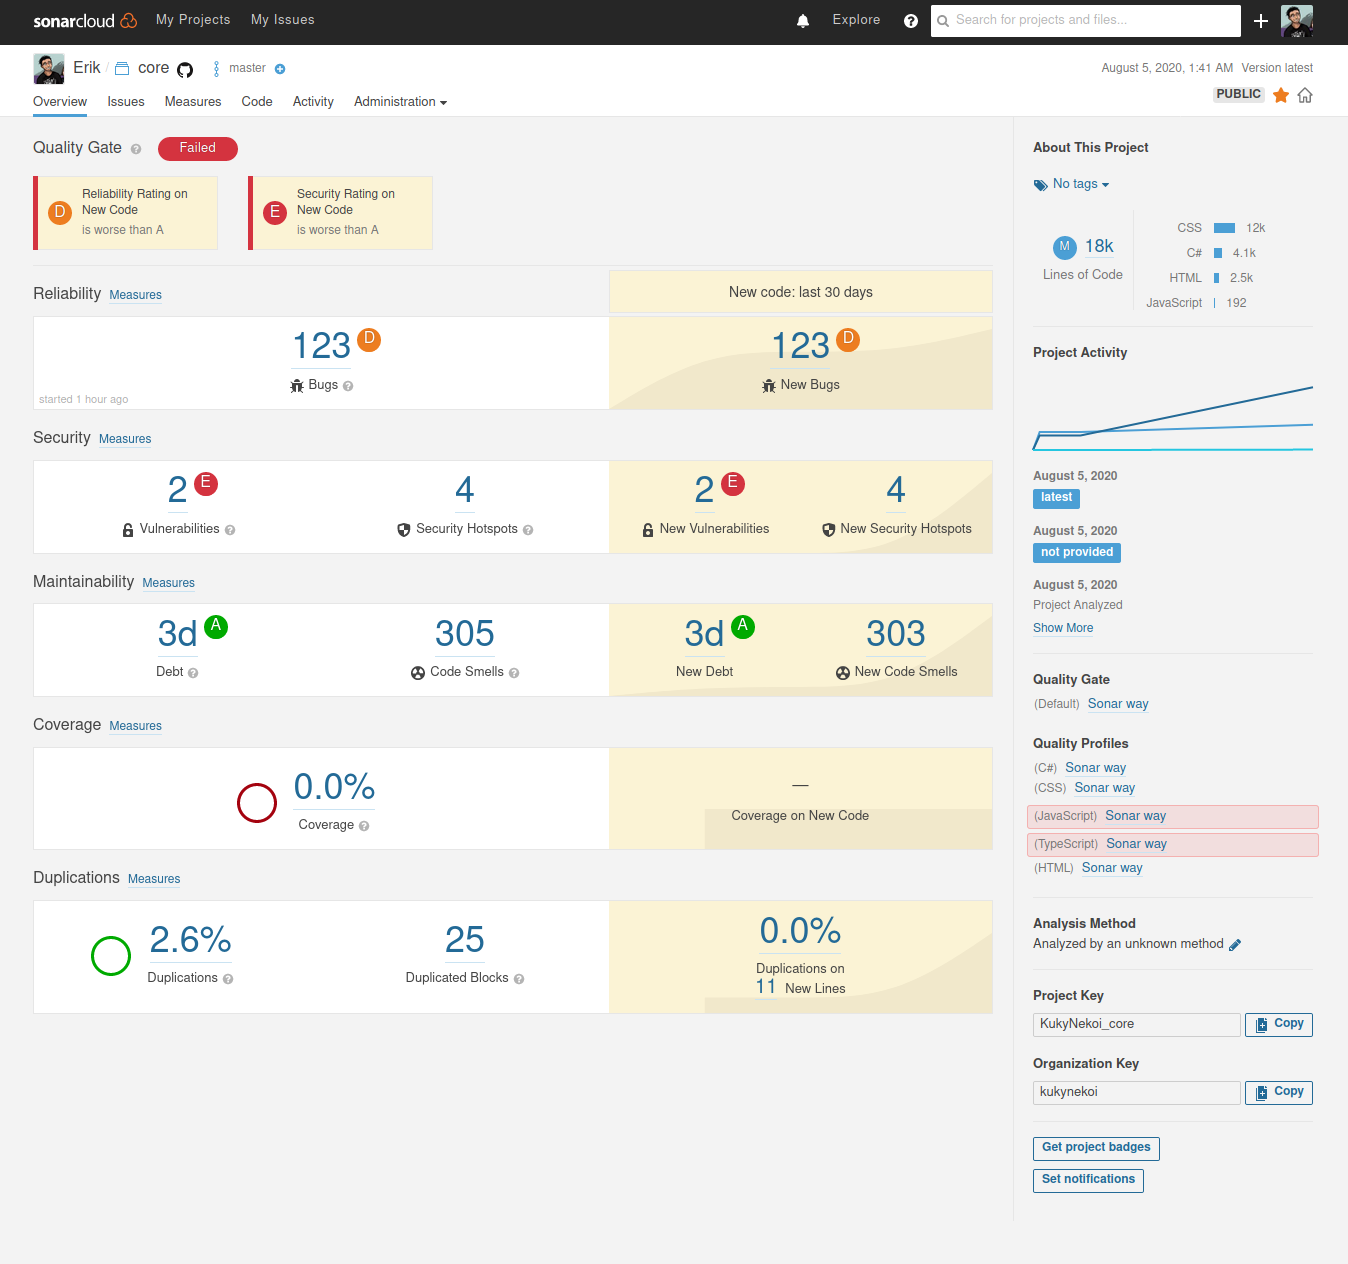
\includegraphics[width=.9\textwidth]{fragments/sonarqube.png}
	\caption{Captura de SonarCloud  }
\end{figure}

Dentro de este análisis estático realizado, se notifican 2 vulnerabilidades en especifico y 4 elementos que requieren atención por implicar problemas de seguridad. Esta herramienta presenta entre otros features, la capacidad de discernir en base a input entregado por la comunidad, el cuando una alerta pertenece a un detalle de código o estilo, es clasificado como tal, lo cual reduce el número de falsos positivos.

\subsubsection{Vulnerabilidades y preocupaciones}

\textbf{Change this code to not construct the path from user-controlled data.} Esta vulnerabilidad fue encontrada en los archivos \texttt{Controllers/FilesController.cs}\footnote{\url{https://sonarcloud.io/project/issues?id=KukyNekoi_core&open=AXO9I4c6uw3EeNfURrkm&resolved=false&types=VULNERABILITY}} y \texttt{Controllers/LinkDocumentFactory.cs}.\footnote{\url{https://sonarcloud.io/project/issues?id=KukyNekoi_core&open=AXO9I4cTuw3EeNfURriv&resolved=false&types=VULNERABILITY}} Para el primero, son valores propagados dentro de la misma declaración del archivo. Sin embargo para el segundo caso, este es un sink de un evento que ocurre en \texttt{Controllers/LinkDocumentFactory.cs} y que es propagado por \texttt{Controllers/RegistriesController.cs}. El problema recae en que hay entradas de usuario que luego de ser propagadas, si estas son construidas de manera adecuada, pueden controlar rutas dentro de la aplicación. 

Para el caso de \texttt{Controllers/FilesController.cs}, este controla la ruta de lectura de un archivo, la cual, si estas no son restringidas pueden provocar una fuga de información. Por otro lado, para \texttt{Controllers/LinkDocumentFactory.cs} si bien el caso es el mismo, este afecta la creación de archivos.

Ambos pueden generar no solo una fuga de información, si no presentan un riesgo latente de inyección de código si no es manejado. Afortunadamente los permisos de ejecución de esos directorios están deshabilitados y los binarios residen en un espacio de usuario aislado del sistema de archivos subyacente. Esto no elimina la fuga de información por medio de la lectura de los archivos.

\textbf{Make sure that hashing data is safe here.} Encontrados en \texttt{Controllers/AuthorizationController.cs}\footnote{\url{https://sonarcloud.io/project/issues?id=KukyNekoi_core&open=AXO9I4dHuw3EeNfURrl2&resolved=false&types=SECURITY_HOTSPOT}}, \url{Models/FileDocumentFactory.cs}\footnote{\url{https://sonarcloud.io/project/issues?id=KukyNekoi_core&open=AXO9I4cguw3EeNfURrjE&resolved=false&types=SECURITY_HOTSPOT}} y \texttt{Models/LinkDocumentFactory.cs}\footnote{\url{https://sonarcloud.io/project/issues?id=KukyNekoi_core&open=AXO9I4cTuw3EeNfURriu&resolved=false&types=SECURITY_HOTSPOT}}, estos problemas hacen referencia a que se está utilizando un algoritmo para realizar el hashing el cual tiene al menos una manera de ser quebrantado. Esto vuelve este mecanismo de hashing inseguro.

Ahora, esto no está bajo la línea de una vulnerabilidad como tal, ya que un algoritmo de hashing puede tener distintos usos, no solamente el cifrado de información. Por ejemplo, la generación automatizada de llaves en base a una cadena de texto determinada, de modo de no colisionar elementos repetidos. Sin embargo, nuestra única consideración al respecto para ser utilizada es sobre la autenticación. Sin embargo, los mecanismos de autenticación no están bajo el control de los desarrolladores, habiendo sido impuestos por el equipo de trabajo detras del desarrollo a la api que se conecta uno de manera remota. Por tanto, no podemos hacer nada en estos casos mas allá de traspasar el riesgo.

\textbf{Make sure that using this pseudorandom number generator is safe here.} Este error se encuentra en \texttt{Controllers/SampleDataController.cs} \footnote{\url{https://sonarcloud.io/project/issues?id=KukyNekoi_core&open=AXO9I4c-uw3EeNfURrko&resolved=false&types=SECURITY_HOTSPOT}} y no tiene mayor relevancia ya que está presente solo en un archivo de prueba el cual no fue eliminado.